\begin{frame}{Two supported hardware platforms}
  Two variants for this course, each using a different hardware
  platform.  \vfill
  \begin{columns}
    \column{0.5\textwidth}
    \begin{center}
      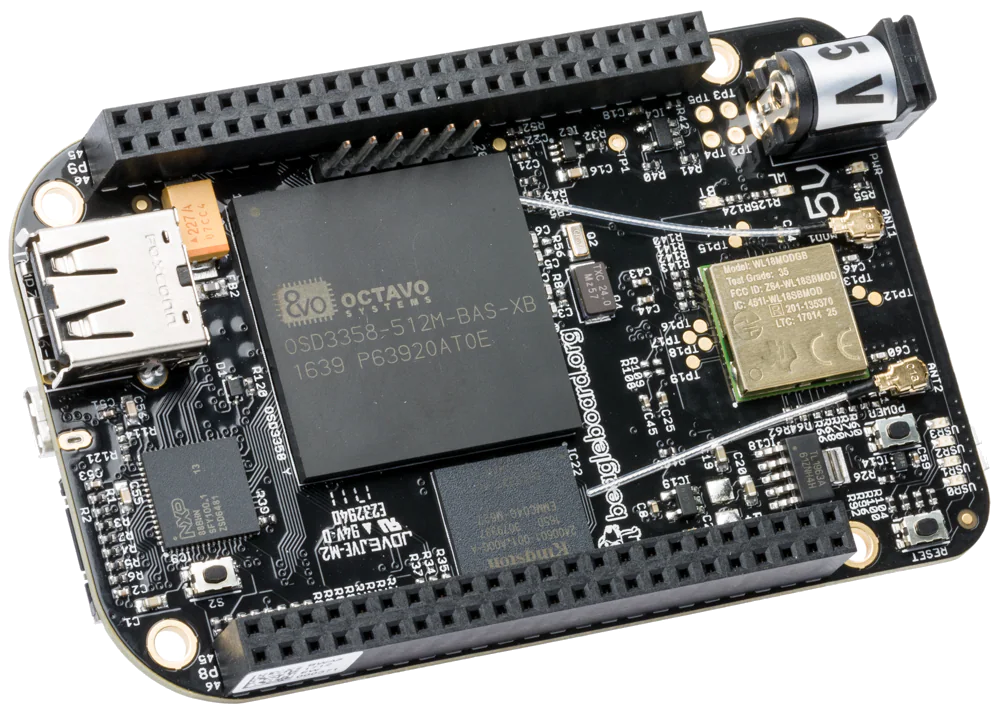
\includegraphics[height=0.4\textheight]{slides/beagleboneblack-board/beagleboneblack.png}
      \newline
      Beaglebone Black
      \newline {\scriptsize \url{https://bootlin.com/doc/training/yocto/}}
    \end{center}
    \column{0.5\textwidth}
    \begin{center}
      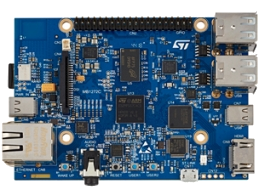
\includegraphics[height=0.4\textheight]{slides/discovery-board-dk1/discovery-board-dk1.png}
      \newline
      STM32MP157D-DK1 Discovery
      \newline {\scriptsize \url{https://bootlin.com/doc/training/yocto-stm32/}}
    \end{center}
  \end{columns}
\end{frame}

\begin{frame}[fragile]{Shopping list: BeagleBone Black Wireless variant}
  \begin{columns}
    \column{0.75\textwidth}
    \begin{itemize}
    \item Beaglebone Black or Beaglebone Black Wireless, USB-A to
      micro B power cable included
      {\fontsize{6}{6}\selectfont
        \url{https://www.mouser.fr/ProductDetail/BeagleBoard-by-GHI/BBBWL-SC-562?qs=k%2Fsw%252B3Yi%2FUbELBjXQpiBUQ%3D%3D}
      }
    \item USB Serial Cable - 3.3 V - female ends (for serial console)
      {\fontsize{6}{6}\selectfont
        \url{https://www.olimex.com/Products/Components/Cables/USB-Serial-Cable/USB-SERIAL-F/}
      }
    \item Nintendo Nunchuk with UEXT connector
      {\fontsize{6}{6}\selectfont
        \url{https://www.olimex.com/Products/Modules/Sensors/MOD-WII/MOD-Wii-UEXT-NUNCHUCK/}
      }
    \item Breadboard jumper wires - Male ends (to connect to Nunchuk)
      {\fontsize{6}{6}\selectfont
        \url{https://www.olimex.com/Products/Breadboarding/JUMPER-WIRES/JW-110x10/}
      }
    \item Micro SD card with 8 GB capacity
    \end{itemize}
    \column{0.25\textwidth}
    \begin{center}
      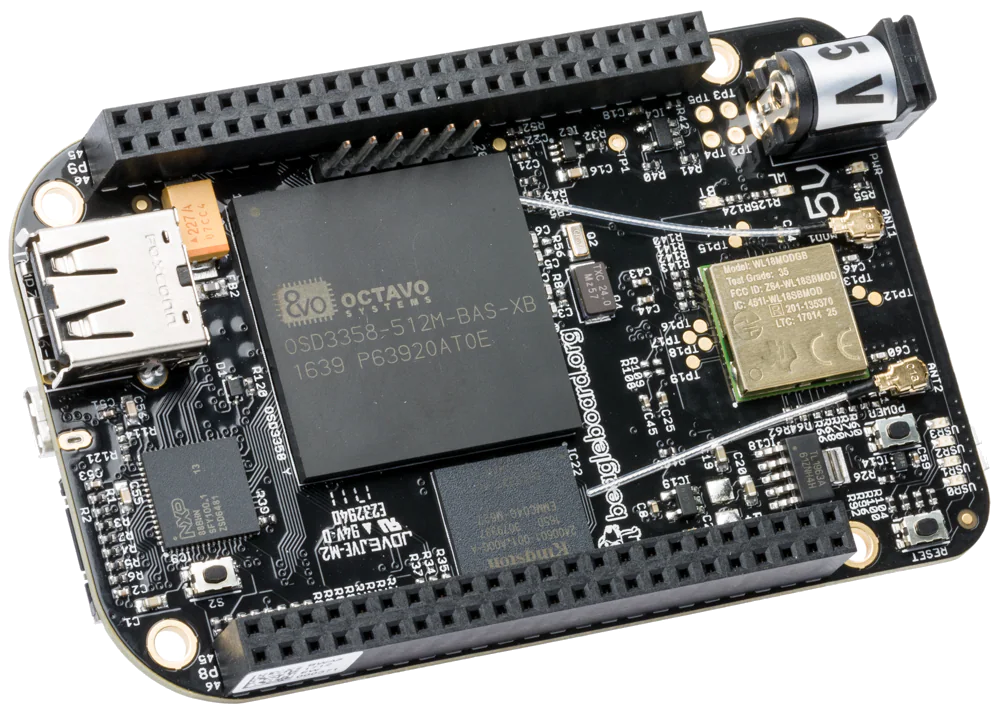
\includegraphics[height=0.2\textheight]{slides/beagleboneblack-board/beagleboneblack.png} \\
      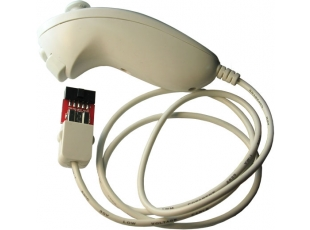
\includegraphics[height=0.2\textheight]{common/nunchuk.jpg} \\
      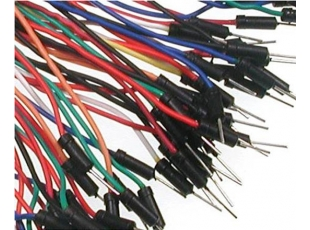
\includegraphics[height=0.15\textheight]{common/jumper-wires.jpg} \\
      %% Source: https://commons.wikimedia.org/wiki/File:SD_card_icon.svg
      
\includegraphics[height=0.15\textheight]{common/sd-card.pdf}
    \end{center}
  \end{columns}
\end{frame}

\begin{frame}[fragile]{Shopping list: STM32MP1 Discovery Kit variant}
  \begin{columns}
    \column{0.75\textwidth}
    \begin{itemize}
    \item STMicroelectronics STM32MP157D-DK1 Discovery kit
      {\fontsize{6}{6}\selectfont
        \url{https://www.st.com/en/evaluation-tools/stm32mp157d-dk1.html#sample-buy}
      }
    \item USB-C cable for the power supply
    \item USB-A to micro B cable for the serial console
    \item Nintendo Nunchuk with UEXT connector
      {\fontsize{6}{6}\selectfont
        \url{https://www.olimex.com/Products/Modules/Sensors/MOD-WII/MOD-Wii-UEXT-NUNCHUCK/}
      }
    \item Breadboard jumper wires - Male ends
      {\fontsize{6}{6}\selectfont
        \url{https://www.olimex.com/Products/Breadboarding/JUMPER-WIRES/JW-110x10/}
      }
    \item Micro SD card with 8 GB capacity
    \end{itemize}
    \column{0.25\textwidth}
    \begin{center}
      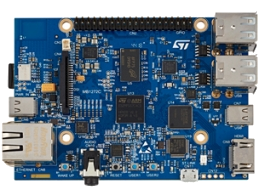
\includegraphics[height=0.2\textheight]{slides/discovery-board-dk1/discovery-board-dk1.png}\\
      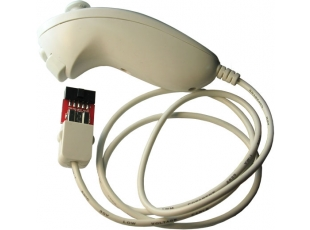
\includegraphics[height=0.2\textheight]{common/nunchuk.jpg} \\
      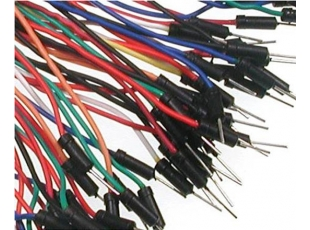
\includegraphics[height=0.15\textheight]{common/jumper-wires.jpg} \\
      %% Source: https://commons.wikimedia.org/wiki/File:SD_card_icon.svg
      
\includegraphics[height=0.15\textheight]{common/sd-card.pdf}
    \end{center}
  \end{columns}
\end{frame}
